%----------------------------------------------------------------------------------------
%	PACKETS AND CONFIGURATION
%----------------------------------------------------------------------------------------

\documentclass[12pt, a4paper]{article}

\usepackage{times} % Times New Roman font
\usepackage{graphicx} % 'graphics' package interface
\usepackage{geometry} % Edit document margins
\usepackage{hyperref} % Table of contents hyperlinks
\usepackage{tcolorbox} % Colored boxes for code
\usepackage[font=small, labelfont=bf]{caption} % Image caption font
\usepackage{longtable} % Build long tables
\usepackage{xurl} % URL breaking

% HELPER PACKAGES (REMOVE IN FINAL) %
\usepackage{blindtext} % Lorem Ipsum
\usepackage{todonotes} % TODOs as useful reminders
\setlength{\marginparwidth}{2cm} % Otherwise todonotes gets angry at me lol
\setuptodonotes{fancyline, color=green!40, shadow} % TODOs options
% HELPER PACKAGES (REMOVE IN FINAL) %

\graphicspath{ {./res/} } % Path to graphics
\hypersetup{    % ToC Hyperlink setup
    colorlinks,
    citecolor=blue,
    filecolor=blue,
    linkcolor=blue,
    urlcolor=blue
}

% Add subsubsubsection
\makeatletter
\newcommand\subsubsubsection{\@startsection{paragraph}{4}{\z@} %
                            {-2.5ex\@plus -1ex \@minus -.25ex} %
                            {1.25ex \@plus .25ex} %
                            {\normalfont\normalsize\bfseries}}
\makeatother
\setcounter{secnumdepth}{4}
\setcounter{tocdepth}{4}

%----------------------------------------------------------------------------------------
%	DOCUMENT
%----------------------------------------------------------------------------------------

\begin{document}

\newgeometry{top=7cm, bottom=2cm} % Setting the margins for the title

% Title
\begin{titlepage}
    \centering
    {\Huge\bfseries Pandemic Information System Model\par} % Project title
    \vspace{1.5cm}
    {\scshape\large Systems and Methods for Big and Unstructured Data \par} % Course
    \vspace{0.5cm}
    {\scshape\large Prof. Marco Brambilla \par} % Professor
    \vspace{1cm}
    {\scshape\large % Description
        Third delivery \par 
        Elasticsearch Project \par 
    }
    \vspace{0.5cm}
    {\slshape\large January 2022 \par} % Date
    \vspace{1cm}
    \linespread{0.8} % Authors interline
    {\large\itshape % Authors
        Avci Oguzhan - \texttt{10557284}\\
        Gentile Nicole - \texttt{10594355}\\
        Rigamonti Davide - \texttt{10629791}\\
        Singh Raul - \texttt{10623232}\\
        Tagliaferri Mattia - \texttt{10572418}
    }
    \vfill
    \begin{figure}[b]
        
\includegraphics[scale=0.6]{polimi.png} % Polimi logo
        \centering
    \end{figure}

    \pagenumbering{gobble} % Remove page number

\end{titlepage}

\newgeometry{bottom=3cm} % Reset the margins
\pagenumbering{arabic} % Reset the page number

\clearpage

% INDEX
{
    \hypersetup{hidelinks}
    \tableofcontents
}

% LIST OF TODOs (REMOVE IN FINAL)
\listoftodos

\clearpage

% Paragraph skip
\setlength{\parskip}{\baselineskip}%
\setlength{\parindent}{0pt}%

% INTRODUCTION
\section{Introduction}

\subsection{Problem Specification}

The idea of the project is to use Elasticsearch to store and analyze data about 
COVID-19 vaccinations in Italy. The data we used can be found in the following 
GitHub repository: \url{https://raw.githubusercontent.com/italia/covid19-opendata-vaccini/master/dati/somministrazioni-vaccini-latest.csv}
and contains data about daily vaccinations divided by region and age range. \\ 
The main goal is to analyze the data in order to build meaningful statistics 
about the vaccinations in Italy; examples can be the total number of doses for each 
vaccine brand, the top regions for vaccine administration etc.

\subsection{Hypoteses}

\begin{itemize}
    \item[] We assumed that the general user doesn't know the italian language, therefore
        all the fields' names contained in the dataset were renamed to an appropriate 
        english translation 
\end{itemize}
  
\clearpage

% DATABASE
\section{Data }

\subsection{Schema description}

\todo{add field descriptions}
\begin{itemize}
    \item Schema for \textbf{vaccines administrations} 
        (somministrazioni-vaccini-latest.csv):
        \begin{itemize}
            \item @timestamp: \emph{date} \\
            \begin{footnotesize}
                elasticsearch timestamp
            \end{footnotesize}
            \item administration\_date (data\_somministrazione): \emph{date [iso8601]} \\
                \begin{footnotesize}
                    date of all the doses' administration
                \end{footnotesize}
            \item supplier (fornitore): \emph{keyword} \\
                \begin{footnotesize}
                    brand of the administrated vaccine, mapped as keyword for easier aggregations
                \end{footnotesize}
            \item area (area): \emph{keyword} \\
                \begin{footnotesize}
                    abbreviation of the region where the administration happened
                \end{footnotesize}
            \item age\_range (fascia\_anagrafica): \emph{keyword} \\
                \begin{footnotesize}
                    age range of the all the subjects given the vaccine, mapped as keyword for queries and aggregations
                \end{footnotesize}
            \item male\_gender (sesso\_maschile): \emph{long} \\
                \begin{footnotesize}
                    total number of male individuals given the vaccine by day and region
                \end{footnotesize}
            \item female\_gender (sesso\_femminile): \emph{long} \\
                \begin{footnotesize}
                    total number of female individuals given the vaccine by day and region
                \end{footnotesize}
            \item first\_dose (prima\_dose): \emph{long} \\
                \begin{footnotesize}
                    total number of first doses
                \end{footnotesize}
            \item second\_dose (seconda\_dose): \emph{long} \\
                \begin{footnotesize}
                    total number of second doses
                \end{footnotesize}
            \item previous\_infection (pregressa\_infezione): \emph{long} \\
                \begin{footnotesize}
                    total number of administrations to subjects with a previous covid-19 infection within 3 and 6 months before the {\it administration date}, therefore needing only one dose 
                \end{footnotesize}
            \item booster\_dose (dose\_addizionale\_booster): \emph{long} \\
                \begin{footnotesize}
                    total number of booster doses
                \end{footnotesize}
            \item total\_doses: \emph{long} \\
                \begin{footnotesize}
                    total number of doses
                \end{footnotesize}
            \item NUTS1\_code (codice\_NUTS1): \emph{keyword} \\
                \begin{footnotesize}
                    European classifications for territorial units. Level: NUTS 1. Mapped as keyword for queries and aggregations
                \end{footnotesize}
            \item NUTS2\_code (codice\_NUTS2): \emph{keyword} \\
                \begin{footnotesize}
                    European classifications for territorial units. Level: NUTS 2. Mapped as keyword for queries and aggregations
                \end{footnotesize}
            \item ISTAT\_region\_code (codice\_regione\_ISTAT): \emph{keyword} \\
                \begin{footnotesize}
                    ISTAT code of the region
                \end{footnotesize}
            \item area\_name (nome\_area): \emph{text} \\
                \begin{footnotesize}
                    name of the region mapped as text for queries with the analyzer
                \end{footnotesize}
        \end{itemize}
    \item Schema for \textbf{population} (platea.csv):
        \begin{itemize}
            \item area (area): \emph{keyword} \\
                \begin{footnotesize}
                    abbreviation of the region/autonomous province
                \end{footnotesize}
            \item area\_name (nome\_area): \emph{text} \\
                \begin{footnotesize}
                    standard name of the area (bilingual name where necessary)
                \end{footnotesize}
            \item age\_range (fascia\_anagrafica): \emph{keyword} \\
                \begin{footnotesize}
                    age range of vaccinable subjects
                \end{footnotesize}
            \item total\_population (totale\_popolazione): \emph{long} \\
                \begin{footnotesize}
                    total population for a given age range
                \end{footnotesize}
        \end{itemize}
    \item Schema for \textbf{healed} (soggetti-guariti.csv):
    \begin{itemize}
        \item area (area): \emph{keyword} \\
            \begin{footnotesize}
                abbreviation of the region/autonomous province
            \end{footnotesize}
        \item area\_name (nome\_area): \emph{text} \\
            \begin{footnotesize}
                standard name of the area (bilingual name where necessary)
            \end{footnotesize}
        \item age\_range (fascia\_anagrafica): \emph{keyword} \\
            \begin{footnotesize}
                age range of healed subjects
            \end{footnotesize}
        \item total\_healed (totale\_healed): \emph{long} \\
            \begin{footnotesize}
                total number of subjects healed up to 6 months ago, for a given age range
                 
            \end{footnotesize}
    \end{itemize}
\end{itemize}

\subsection{Dataset description}

The dataset contains data about COVID-19 vaccinations in Italy. \\
For each day, region and age range we have information about the number of vaccinated 
people (male and female), the number of 1st, 2nd and booster doses and information 
about the number of people who was previously infected. \\
We decided to integrate this data using the ‘platea.csv’ dataset that can be found 
in the specified repository; it contains data about the population for each region 
and each age range. \\ 
We also used information about the number of healed people in each region that can be 
found in ‘soggetti-guariti.csv’ present in the same repository.

%QUERIES
\subsection{Queries}

\subsubsection{Number of daily vaccines for each dose}
Total number of first, second and booster doses administred in each date.
\begin{tcolorbox}[fontupper=\scriptsize]
    \begin{verbatim}
GET /index-vaccines_administrations/_search
{
"size": 0, 
  "aggs": {
    "Administration Date": {
      "terms": {
        "field": "administration_date",
        "size": 370
      },
      "aggs": {
        "totalFirstDoses": {
          "sum": {
            "field": "first_dose"
          }
        },        
        "totalSecondDoses": {
          "sum": {
            "field": "second_dose"
          }
        },        
        "totalBoosters": {
          "sum": {
            "field": "booster_dose"
          }
        }
      }
    }
  } 
}

    \end{verbatim}
\end{tcolorbox}

\noindent

\subsubsection{Number of doses per gender in each region}
Total doses administred to men and women in each region. 
\begin{tcolorbox}[fontupper=\scriptsize]
    \begin{verbatim}
GET /index-vaccines_administrations/_search
{
"size": 0, 
  "aggs": {
    "Region": {
      "terms": {
        "field": "area",
        "size": 21
      },
      "aggs": {
        "totalWomenDoses": {
          "sum": {
            "field": "female_gender"
          }
        },        
        "totalMenDoses": {
          "sum": {
            "field": "male_gender"
          }
        }
      }
    }
  } 
}

    \end{verbatim}
\end{tcolorbox}

\noindent

\subsubsection{Number of vaccines per dose number in each region}
Total number of first, second, booster and total doses administred in each region.
\begin{tcolorbox}[fontupper=\scriptsize]
    \begin{verbatim}
GET /index-vaccines_administrations/_search
{
"size": 0, 
  "aggs": {
    "Region": {
      "terms": {
        "field": "area",
        "size": 21
      },
      "aggs": {
        "totalFirstDoses": {
          "sum": {
            "field": "first_dose"
          }
        },        
        "totalSecondDoses": {
          "sum": {
            "field": "second_dose"
          }
        },        
        "totalBoosters": {
          "sum": {
            "field": "booster_dose"
          }
        },        
        "totalDoses": {
          "sum": {
            "field": "total_doses"
          }
        }
      }
    }
  } 
}

    \end{verbatim}
\end{tcolorbox}

\noindent

\subsubsection{Number of doses for each vaccine supplier}
Total doses for each vaccine supplier (Pfizer/BioNTech, Moderna, Vaxzevria (AstraZeneca), Janssen, Pfizer Pediatrico).
\begin{tcolorbox}[fontupper=\scriptsize]
    \begin{verbatim}
GET /index-vaccines_administrations/_search
{"size":0,
  "aggs": {
    "supplier": {
      "terms": {
        "field": "supplier"
      },
      "aggs": {
        "total_doses" : { "sum" : {
          "field": "total_doses"
          }
        }
      }
    }
  }
}

    \end{verbatim}
\end{tcolorbox}

\noindent

\subsubsection{Number of doses for each NUTS1 zone}
Total number of doses administred in each NUTS1 zone (ITC= NorthWest, ITH = NorthEast, ITI = Center, ITF = South, ITG = Isles)
\begin{tcolorbox}[fontupper=\scriptsize]
    \begin{verbatim}
GET /index-vaccines_administrations/_search
{"size":0,
  "aggs": {
    "by_NUTS1": {
      "terms": {
        "field": "NUTS1_code"
      },
      "aggs": {
        "total_doses" : { "sum" : {
          "field": "total_doses"
          }
        }
      }
    }
  }
}
    \end{verbatim}
\end{tcolorbox}

\noindent

\subsubsection{Number of people with previous infection by region}
Total number of people who was infected by Covid-19 before the vaccination in each region.
\begin{tcolorbox}[fontupper=\scriptsize]
    \begin{verbatim}
GET /index-vaccines_administrations/_search
{
  "size":0,
  "aggs": {
    "Region": {
      "terms": {
        "field": "area"
      },
      "aggs": {
        "People with previous infection": {
          "sum": {
            "field": "previous_infection"
          }
        }
      }
    }
  }
}
    \end{verbatim}
\end{tcolorbox}

\noindent

\subsubsection{Number of doses for each age group}
Total number of doses administred to each age range ('05-11', '12-19', '20-29', '30-39', '40-49', '50-59', '60-69', '70-79', '80-89',
       '90+').
\begin{tcolorbox}[fontupper=\scriptsize]
    \begin{verbatim}
GET /index-vaccines_administrations/_search
{"size":0,
  "aggs": {
    "by_age": {
      "terms": {
        "field": "age_range"
      },
      "aggs": {
        "total_doses" : { "sum" : { 
          "field": "total_doses"
          }
        }
      }
    }
  }
}

    \end{verbatim}
\end{tcolorbox}

\noindent

\subsubsubsection{Grouping by age range and region}
Total number of doses administred to each age range in each region.
\begin{tcolorbox}[fontupper=\scriptsize]
    \begin{verbatim}
GET /index-vaccines_administrations/_search
{"size":0,
  "aggs": {
    "genres_and_products": {
      "multi_terms": {
        "terms": [{
          "field": "age_range" 
        }, {
          "field": "area"
        }], 
        "size": 1000
      },
      "aggs": {
        "total_doses" : { "sum" : { 
          "field": "total_doses"
          } 
        }
      }
    }
  }
}

    \end{verbatim}
\end{tcolorbox}

\noindent

\subsubsection{Number of average doses per region}
Average umber of administred doses in each region.
\begin{tcolorbox}[fontupper=\scriptsize]
    \begin{verbatim}
GET /index-vaccines_administrations/_search
{"size":0,
  "aggs": {
    "Region": {
      "terms": {
        "field": "area"
      },
      "aggs": {
        "avg_doses" : { "avg": {
          "field": "total_doses"
        } } 
      }
    }
  }
}

    \end{verbatim}
\end{tcolorbox}

\noindent

\subsubsection{Number of doses for age group and vaccine supplier}
Total number of doses divided by age group and vaccine supplier.
\begin{tcolorbox}[fontupper=\scriptsize]
    \begin{verbatim}
GET /index-vaccines_administrations/_search
{
  "size": 0,
  "track_total_hits": true,
  "aggs": {
    "age_groups_types": {
      "composite": {
        "sources": [{
          "fascia_anagrafica": {
            "terms": { 
              "field": "age_range"
            }
          }
        }, {
          "supplier": {
            "terms": { 
              "field": "supplier"
            }
          }
        }], 
        "size": 10000
      },
      "aggs": {
        "total_vaccines": {
          "sum": {
            "field": "total_doses"
          }
        }
      }
    }
  }
}
    \end{verbatim}
\end{tcolorbox}

\noindent

\subsubsection{Number of booster doses for age range}
Total number of booster doses for each age range.
\begin{tcolorbox}[fontupper=\scriptsize]
    \begin{verbatim}
GET /index-vaccines_administrations/_search
{
  "size": 0,
  "aggs": {
    "age_groups": {
      "terms": { 
        "field": "age_range" 
      },
      "aggs": {
        "boosters_per_group": {
          "sum": {
            "field": "booster_dose"
          }
        }
      }
    }
  }
}
    \end{verbatim}
\end{tcolorbox}

\noindent

\subsubsection{Top 10 dates with most vaccinations}
Top 10 dates having the highest number of administred doses.
\begin{tcolorbox}[fontupper=\scriptsize]
    \begin{verbatim}
GET index-vaccines_administrations/_search
{
  "size": 0,
  "aggs": {
    "dates": {
      "terms": { 
        "field": "administration_date" 
      },
      "aggs": {
        "sum_vaccinations": {
          "sum": {
            "field": "total_doses"
          }
        },
        "dates_sort": {
          "bucket_sort": {
            "sort": [
              { "sum_vaccinations": { "order" : "desc" } }
            ],
            "size": 10
          }
        }
      }
    }
  }
}
    \end{verbatim}
\end{tcolorbox}

\noindent

\subsubsection{Search by region name}
Returns information about vaccines in the specified region.
\begin{tcolorbox}[fontupper=\scriptsize]
    \begin{verbatim}
GET /index-vaccines_administrations/_search
{
  "query": {
    "match": {
          "area_name": "Val d'aosta"
    }
  }
}
    \end{verbatim}
\end{tcolorbox}
\noindent

\subsection{Commands}

\subsubsection{Add entries for a given day}
Add a new document in the dataset.
\begin{tcolorbox}[fontupper=\scriptsize]
    \begin{verbatim}
POST /index-vaccines_administrations/_doc/
 {    
    "area" : "FVG",
    "area_name" : "Friuli-Venezia Giulia",
    "second_dose" : 0,
    "previous_infection" : 1,
    "administration_date" : "2022-01-03",
    "NUTS1_code" : "ITH",
    "ISTAT_region_code" : 6,
    "male_gender" : 3,
    "first_dose" : 2,
    "age_range" : "30-39",
    "supplier" : "Moderna",
    "total_doses" : 3,
    "booster_dose" : 0,
    "NUTS2_code" : "ITH4",
    "female_gender" : 0,
    "total_doses" : 3
}
    \end{verbatim}
\end{tcolorbox}

\noindent

\subsubsection{Remove entries from a given day}
Remove all documents in the specified date.
\begin{tcolorbox}[fontupper=\scriptsize]
    \begin{verbatim}
POST /index-vaccines_administrations/_delete_by_query
{
  "query": {
    "match": {
      "administration_date": "2022-01-03"
    }
  }
}
    \end{verbatim}
\end{tcolorbox}

\noindent

\clearpage

\section{Data Visualization with Kibana}
We used the dashboard to give a visual representation of the most meaningful queries. \\
In order to use this dashboard, you need to create three indexes (one for each csv file) and name them respectively: "index-vaccines\_administrations", "index-population" and "index-healed". \\
Then, you need to add in the "index-patterns" section an aggregate index named "index"; it will create an overall "index-*" that combines all the indexes allowing you to see some visualizations in the dashboard. 

\subsection{Screenshots}
We used a control panel to allow to filter the results of the other elements of the dashboard based on region, vaccine supplier and age range.
\begin{figure}[ht]
  \centering
  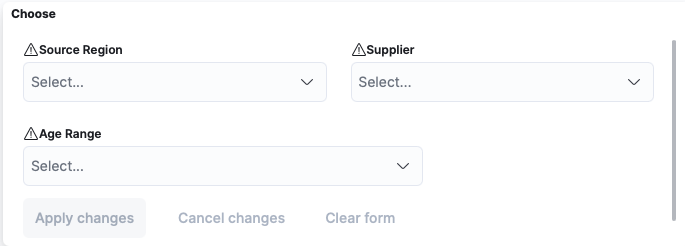
\includegraphics[width=.9\linewidth]{img (2).png}
\end{figure}

\subsubsection{Map visualization}
It allows to represent a dynamic map of Italy divided in regions. By default it shows the number of administred first doses in each region. \\ 
By hovering over a region, it shows a description of the number of vaccinations for each type (first, second, booster doses and so on) administered by that region.
\begin{figure}[ht]
  \centering
  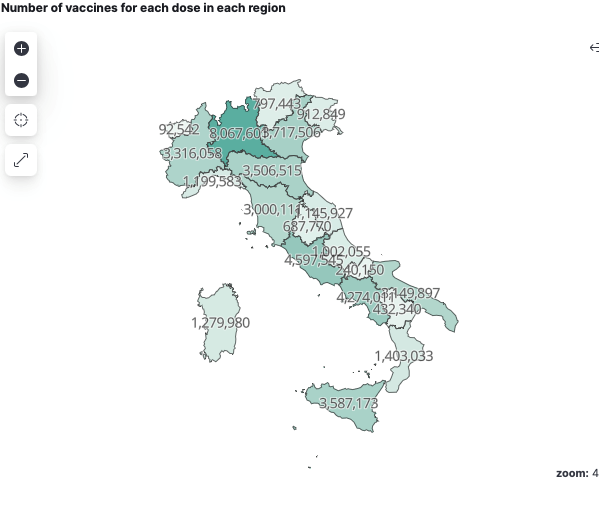
\includegraphics[width=1\linewidth]{img (4).png}
\caption*{Map of Italy (left); result of hovering (right)}
\end{figure}

\subsubsection{Pie Chart}
It represents the percentage of doses for each vaccine brand and for each NUTS1 over the total administred vaccines.
\begin{figure}[ht]
  \centering
  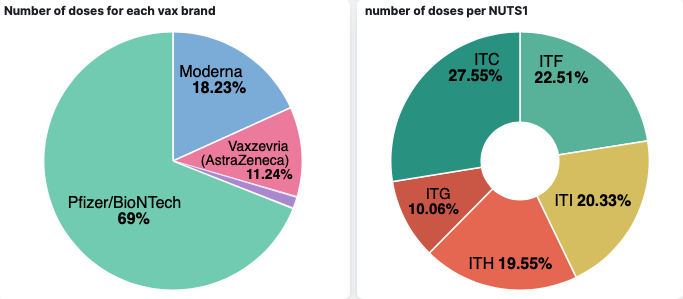
\includegraphics[width=1\linewidth]{img (7).png}
\caption*{Pie charts}
\end{figure}

\subsubsection{Metric Visualization}
It represents the percentage of people with at least one/two ore three doses and the number of people who healed from Covid-19 in the selected region (or in Italy if none is selected).
\begin{figure}[ht]
  \centering
  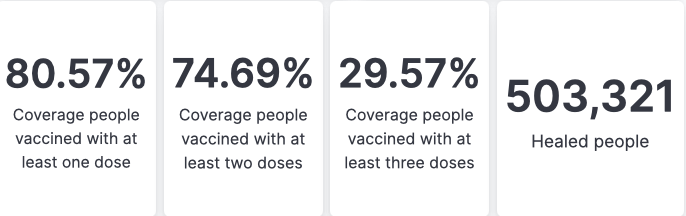
\includegraphics[width=.8\linewidth]{img (8).png}
\caption*{Metric visualization}
\end{figure}

\subsubsection{Number of vaccines by genre}
Represents a comparison between the total number of vaccines done by males and females, in each week from the starting date selected. By hovering with the mouse, a more detailed percentage is shown.
\begin{figure}[ht]
  \centering
  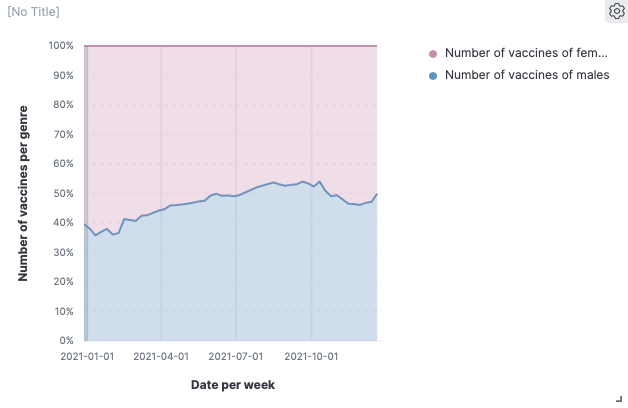
\includegraphics[width=.8\linewidth]{img (9).png}
\caption*{Number of vaccines by genre}
\end{figure}

\subsubsection{Average number of vaccines by region}
Represents the average number of vaccines administred in each region.
\begin{figure}[ht]
  \centering
  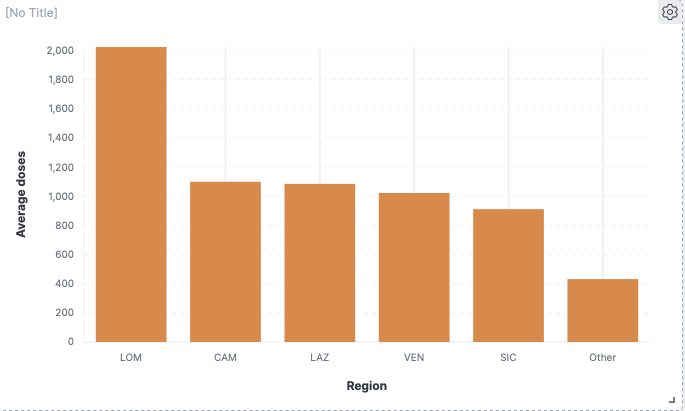
\includegraphics[width=.8\linewidth]{img (10).png}
\caption*{Average number of vaccines by region}
\end{figure}

\subsubsection{Number of 1st, 2nd and booster doses per week}
It shows a graph that, for each week from the starting date selected, represents the trend of the total doses administered by type (1st, 2nd or booster doses).
\begin{figure}[ht]
  \centering
  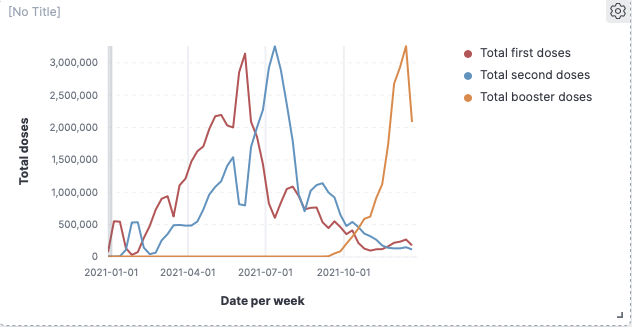
\includegraphics[width=.8\linewidth]{img (11).png}
\caption*{Number of 1st, 2nd and booster doses}
\end{figure}

\subsubsection{Total number of vaccines by date}
It shows the total number of administred doses in each day.
\begin{figure}[ht]
  \centering
  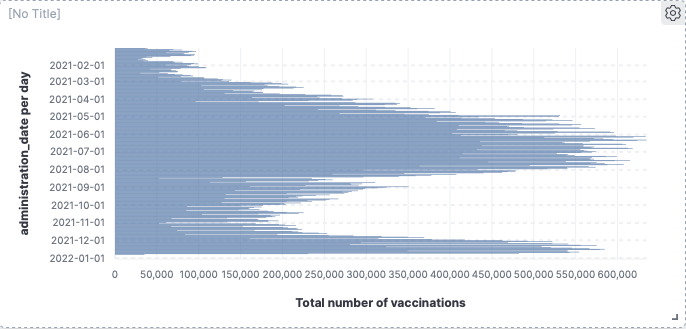
\includegraphics[width=.8\linewidth]{img (12).png}
\caption*{Total number of vaccines by date}
\end{figure}


\clearpage

%OPTIONAL POINT N°2
\section{Other features in HBase} 

We deciced to use \emph{HBase} as an alternative NoSQL DBMS in order to implement some 
additional features.vfill \\
\emph{HBase} is a column-oriented DBMS usually utilized in the context of the 
\emph{Apache Hadoop} framework, it can be run locally using \emph{Apache Zookeeper} or 
by installing \emph{Hadoop} and running \emph{HBase} on top of \emph{HDFS}.

\subsection{Input Data Preparation}

In order to import data into \emph{HBase}, the first step is to eliminate the labels 
from the csv file containing raw data. \\
In our case the file has been renamed as \emph{vaccines\_administrations\_latest.csv} 
and a \\ unique ID generated using \emph{Python} \texttt{uuid.uuid4()} function 
(from the \texttt{uuid} library) has been added as the first item for each row since
HBase expects a row key in that particular position. \\ 
The unique ID was generate in this way since an incremental sequential number as a 
row key is not recommended according to the \emph{HBase} documentation. 

\noindent
Once we have the data in CSV format, we have to store it in a path from where 
\emph{HBase} can access it. \\
If we want to load the file using Hadoop, we will have to copy the file to the 
\emph{HDFS} location, this can be done using the command:
\begin{footnotesize}
  \begin{itemize}
    \item[] \texttt{hadoop fs -copyFromLocal <LOCAL\_PATH>  <HDFS\_PATH>} 
  \end{itemize}
\end{footnotesize}

\subsection{Storing data into HBase}

\begin{footnotesize}
  \begin{itemize}
    \item[] \texttt{create 'vaccines\_administrations', \{NAME => '\_date'\}, \\
      \{NAME => '\_type'\}, \{NAME => 'region'\}, \\
      \{NAME => 'stats'\}, \{NAME => 'doses'\}, \{NAME => 'nuts'\}} 
  \end{itemize}
\end{footnotesize}
This command will create an \emph{HBase} table in order to store the data. \\
Notice that we are creating five column families for some of the columns of the CSV file,
this is done for accessing and querying the data in a more easier and flexible way using
\emph{Apache Drill}. 

\vfill % Aesthetic purpose

\begin{footnotesize}
  \begin{itemize}
    \item[] \texttt{./hbase org.apache.hadoop.hbase.mapreduce.ImportTsv \\
      -Dimporttsv.separator=',' \\
      -Dimporttsv.columns=HBASE\_ROW\_KEY,\_date:administration\_date, \\
        \_type:supplier,region:area,stats:age\_range,stats:male\_gender, \\
        stats:female\_gender,doses:first\_dose,doses:second\_dose, \\
        doses:previous\_infection,doses:booster\_dose,nuts:NUTS1\_code, \\
        nuts:NUTS2\_code,region:ISTAT\_region\_code,region:area\_name \\
      vaccines\_administrations \\
      <PATH>} 
  \end{itemize}
\end{footnotesize}
Once we submit this command a \emph{MapReduce} that will import the CSV file into the 
HBase table that we created will start. \\
Each column of the CSV file is mapped into the respective column family.  \\
\texttt{<PATH>} needs be changed to the HDFS path if we are using \emph{Hadoop} or to 
the local path of the CSV file if we are using \emph{Zookeeper}. \\
The output should resemble the following: 

\begin{figure}[ht]
  \centering
  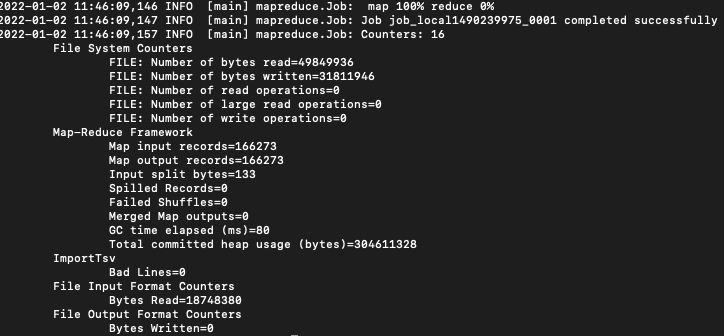
\includegraphics[width=\linewidth]{hbase_import.png}
\end{figure}

\subsection{Querying HBase}

For querying \emph{HBase} we decided to use \emph{Apache Drill}, this means that our
queries will be written in SQL and can benefit from all the extensions that the 
framework provides. \\
To be able to query an \emph{HBase} database, after running \emph{Apache Drill} in 
embedded mode, we will have to go to the storage section and enable \emph{HBase}.  

\noindent
The translation of some Elasticsearch queries with sample screenshots of possible results
will be provided here, a more complete selection of queries will be provided separately.

\subsubsection{Number of daily vaccines for each dose}

\begin{tcolorbox}[fontupper=\scriptsize]
  \begin{verbatim}
SELECT CONVERT_FROM(vaccines_administrations._date.administration_date, 'UTF8') 
        AS date_time,
  SUM(CAST(vaccines_administrations.doses.first_dose AS INT)) 
          AS number_of_daily_vaccines_first_dose,
  SUM(CAST(vaccines_administrations.doses.second_dose AS INT)) 
          AS number_of_daily_vaccines_second_dose,
  SUM(CAST(vaccines_administrations.doses.booster_dose AS INT)) 
          AS number_of_daily_vaccines_booster_dose
FROM vaccines_administrations
GROUP BY date_time
  \end{verbatim}
\end{tcolorbox}

\noindent
Possible result:
\begin{figure}[ht]
  \centering
  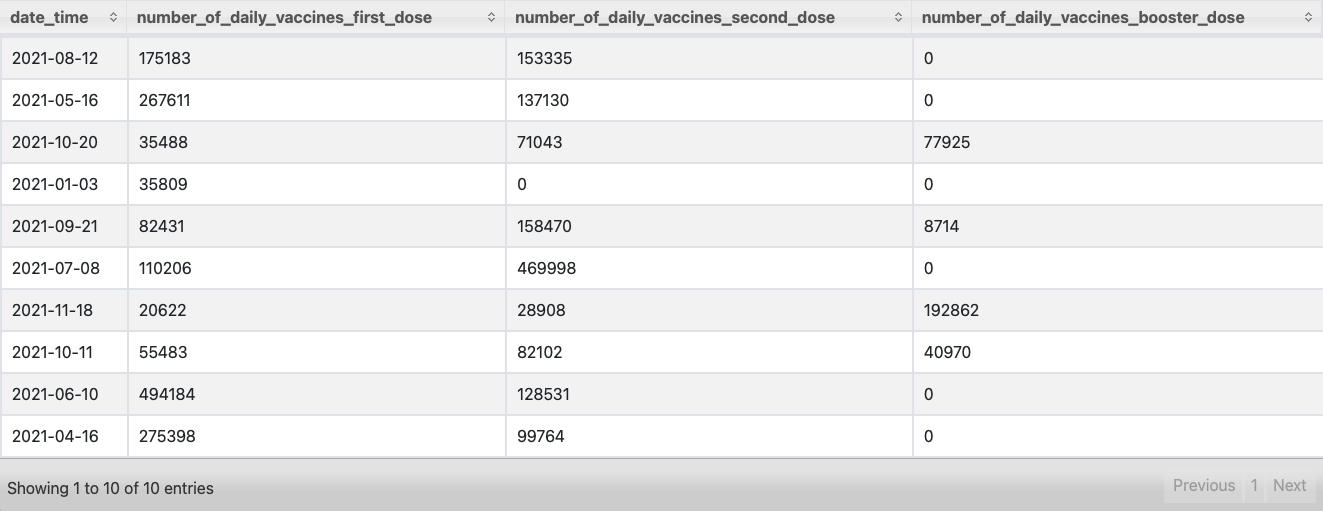
\includegraphics[width=\linewidth]{hbase_query_1.png}
\end{figure}

\subsubsection{Number of doses for each vaccine supplier}

\begin{tcolorbox}[fontupper=\scriptsize]
  \begin{verbatim}
SELECT CONVERT_FROM(vaccines_administrations._type.supplier, 'UTF8') 
        AS supplier,
  SUM(CAST(vaccines_administrations.doses.first_dose AS INT)   + 
      CAST(vaccines_administrations.doses.second_dose AS INT)  + 
      CAST(vaccines_administrations.doses.booster_dose AS INT) +
      CAST(vaccines_administrations.doses.previous_infection AS INT)) 
          AS total_doses
FROM vaccines_administrations
GROUP BY supplier
  \end{verbatim}
\end{tcolorbox}

\clearpage % Aesthetic purpose

\noindent
Possible result:
\begin{figure}[ht]
  \centering
  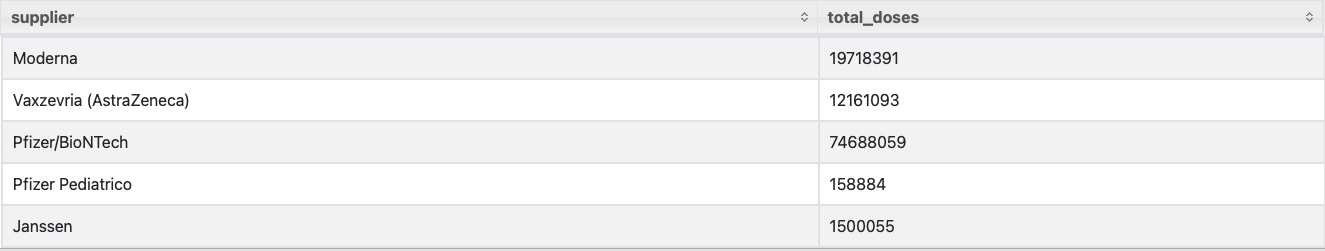
\includegraphics[width=\linewidth]{hbase_query_2.png}
\end{figure}

\subsubsection{Top 10 dates with most vaccinations}

\begin{tcolorbox}[fontupper=\scriptsize]
  \begin{verbatim}
SELECT CONVERT_FROM(vaccines_administrations._date.administration_date, 'UTF8') 
        AS administration_date,
  SUM(CAST(vaccines_administrations.doses.first_dose AS INT)   + 
      CAST(vaccines_administrations.doses.second_dose AS INT)  + 
      CAST(vaccines_administrations.doses.booster_dose AS INT) +
      CAST(vaccines_administrations.doses.previous_infection AS INT)) 
          AS total_vaccinations
FROM vaccines_administrations
GROUP BY administration_date
ORDER BY total_vaccinations ASC
LIMIT 10;
  \end{verbatim}
\end{tcolorbox}

\noindent
Possible result:
\begin{figure}[ht]
  \centering
  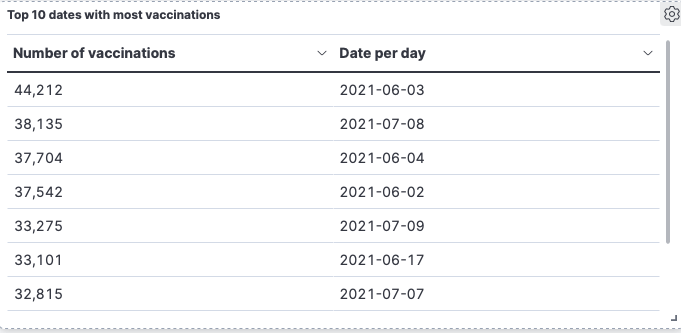
\includegraphics[width=\linewidth]{hbase_query_3.png}
\end{figure}

\clearpage

% REFERENCES AND SOURCES
\section{References and sources}

In order to develop this project, the following tools were used:

\begin{itemize}
    \item Elasticsearch and Kibana in order to store, query and visualize data;
    \item HBase, HDFS, Hadoop, Apache Drill and Zookeeper as an alternative NoSQL 
      framework for some features;
    \item Python as a mean to easily modify and prepare files for import;
    \item \LaTeX~to write the report;
    \item Github as a versioning and collaboration mean;
    \item \url{https://github.com/italia/covid19-opendata-vaccini} \\
        as a source of updated and real data about vaccinations in Italy.
\end{itemize}

\clearpage

\end{document}
